%%%%%%%%%%%%%%%%%%%%%%%%%%%%%%%%%%%%%%%%%%%%%%%%%%%%%%%%%%%%%%%%%%%%%%
% LaTeX Template: Beamer arrows
%
% Source: http://www.texample.net/
% Feel free to distribute this template, but please keep the
% referal to TeXample.net.
% Date: Nov 2006
% 
%%%%%%%%%%%%%%%%%%%%%%%%%%%%%%%%%%%%%%%%%%%%%%%%%%%%%%%%%%%%%%%%%%%%%%
% How to use writeLaTeX: 
%
% You edit the source code here on the left, and the preview on the
% right shows you the result within a few seconds.
%
% Bookmark this page and share the URL with your co-authors. They can
% edit at the same time!
%
% You can upload figures, bibliographies, custom classes and
% styles using the files menu.
%
% If you're new to LaTeX, the wikibook is a great place to start:
% http://en.wikibooks.org/wiki/LaTeX
%
%%%%%%%%%%%%%%%%%%%%%%%%%%%%%%%%%%%%%%%%%%%%%%%%%%%%%%%%%%%%%%%%%%%%%%

\documentclass{beamer} %
\usetheme{CambridgeUS}
\usepackage[utf8]{inputenc}
\usefonttheme{professionalfonts}
\usepackage{times}
\usepackage{tikz}
\usepackage{amsmath}
\usepackage{verbatim}
\usetikzlibrary{arrows,shapes}

\author{Author}
\title{Presentation title}

\begin{document}

\title[INFO-F-410 - Traffic Light Control]{\textbf{Traffic Light Control} \\INFO-F-410 -- Embedded Systems Design} % The short title appears at the bottom of every slide, the full title is only on the title page

\author{Jamal \textsc{Ben Azouze}, Marien \textsc{Bourguignon}, Nicolas \textsc{De Groote}, \\Simon \textsc{Picard}, Arnaud \textsc{Rosette}, Gabriel \textsc{Ekanga}}
\institute[ULB] % Your institution as it will appear on the bottom of every slide, may be shorthand to save space
{
Université Libre de Burxelles \\ % Your institution for the title page
\medskip
\textit{Département d'Informatique} % Your email address
}
\date{4 Juin 2015} % Date, can be changed to a custom date

\begin{frame}
\titlepage % Print the title page as the first slide
\end{frame}

\begin{frame}{Sommaire}
\tableofcontents % Throughout your presentation, if you choose to use \section{} and \subsection{} commands, these will automatically be printed on this slide as an overview of your presentation
\end{frame}

\section{Introduction}
\begin{frame}{Introduction}

\end{frame}

\section{Acteurs et automates}
\begin{frame}{Acteurs et automates}

\end{frame}

\section{Condition de succès}
\begin{frame}[fragile]{Condition de succès}
\begin{block}{1. Un piéton ne se fait pas écraser}
\begin{verbatim}
form_1 = 
control: A[] not(PedestrianGeneratorEast.Cross && 
(
    CarGeneratorEast.Go || 
    (
        CarGeneratorWest.Go && queue[W][0] == U
    ) || (
        CarGeneratorSouth.Go && queue[S][0] == R
    )))
\end{verbatim}
\end{block}

\end{frame}
\begin{frame}[fragile]{Condition de succès}
\centering
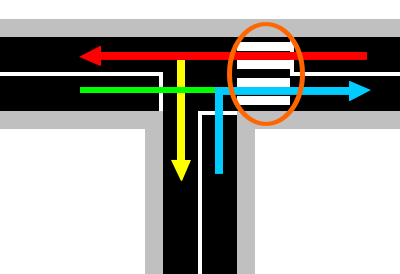
\includegraphics[scale=0.8]{images/pietonCollision.png}

\end{frame}


\begin{frame}[fragile]{Condition de succès}
\begin{block}{2. Il n'y a pas de collision entre les voitures}
\begin{verbatim}
form_2 = 
Control: A[] not
(
    CarGeneratorWest.Go && queue[W][0] == U && 
    ((
        CarGeneratorEast.Go && queue[E][0] == L
    ) || (
        CarGeneratorSouth.Go && 
        ( queue[S][0] == L || queue[S][0] == R )
    ))
) || (
    CarGeneratorWest.Go && queue[W][0] == R 
    && CarGeneratorEast.Go && queue[E][0] == L
)
\end{verbatim}
\end{block}

\end{frame}
\begin{frame}[fragile]{Condition de succès}
\centering
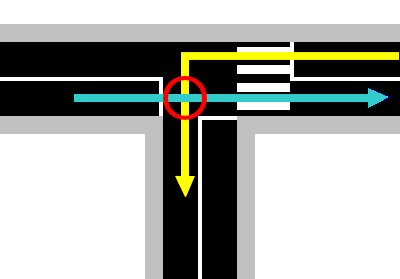
\includegraphics[scale=0.8]{images/exempleCollision.png}

\end{frame}


\begin{frame}[fragile]{Condition de succès}
\begin{block}{3. Un piéton n'attend pas infiniment}
\begin{verbatim}
form_3 = 

control: A[] not (PedestrianGeneratorEast.Broken)
\end{verbatim}
\end{block}

\begin{block}{4. Une voiture n'attend pas infiniment}
\begin{verbatim}
form_4 = 

control: A[] not (CarGeneratorEast.Broken ||
                  CarGeneratorSouth.Broken ||
                  CarGeneratorWest.Broken)
\end{verbatim}
\end{block}

\end{frame}

\begin{frame}[fragile]{Condition de succès}
\begin{block}{Condition finale}
\begin{verbatim}
control: A[] not (
    form_1 || form_2 || form_4 ||form_4
)
\end{verbatim}
\end{block}
\end{frame} 

\section{Simuation}
\begin{frame}{Simuation}

\end{frame}

\section{Conclusion}
\begin{frame}{Conclusion}

\end{frame}
\end{document}